\section{Gaussian Process Modeling}
\label{gp}
The study of Gaussian processes is rich and deep and more completely covered by 
other resources, such as \cite{rasmussen2006gaussian}. Here only the barest of 
introductions to this topic are given as motivated by the regression problem at
hand. For nuclear fuel cycle benchmark analysis, Gaussian processes will be used
to form a model of the metric time series over all $S$ simulators. 

A Gaussian process is defined by mean and covariance functions. 
In general, these functions may be parameterized by many independent and 
many dependent variables.  However, for purpose of this paper, a single 
independent parameter, time, is sufficient to demonstrate the method without 
loss of generality.  
Here, the mean function $\mu(t)$ is taken to be the expectation value $\E$ of 
the input functions, which here are the time series for all simulators. The
covariance function $k(t, t^\prime)$ is the expected value of the input 
functions to the mean. Symbolically, 
\begin{equation}
\label{mean-func}
\mu(t) = \E\left[m_s^i(t)\right] = \E\left[m_0^i(t), m_1^i(t), \ldots\right]
\end{equation}
\begin{equation}
\label{covar-func}
k(t, t^\prime) = \E\left[(m_s^i(t) - \mu(t))(m_s^i(t^\prime) - \mu(t^\prime))\right]
\end{equation}
The Gaussian process $\GP$ thus approximates the metric given information 
from all simulators. This is denoted either using functional or operator notation as follows:
\begin{equation}
\label{gp-def-approx}
m_*^i(t) \approx \GP\left(\mu(t), k(t, t^\prime)\right) \equiv \GP m_s^i
\end{equation}
Let $*$ indicate that the variable is associated with  
the model, rather than any of the raw simulator data.


For Gaussian process regression, a functional form for the covariance 
$k(t, t^\prime)$ needs to be provided.
This is sometimes called the kernel function and contains the free parameters 
for the regression, also called hyperparameters. How the hyperparameters are 
defined is 
tied to the definition of the kernel function itself. The values for the 
hyperparameters are determined
via optimization of the maximal likelihood of the value of the metric function.
While there are many possible kernels, a standard and generically applicable one 
is the exponential squared kernel, as seen in Equation \ref{exp2-kernel}:
\begin{equation}
\label{exp2-kernel}
k(t, t^\prime) = \sigma^2 \exp\left[-\frac{1}{2\ell}(t - t^\prime)^2 \right]
\end{equation}
Here, the length scale $\ell$ and the signal variance $\sigma^2$ are the 
hyperparameters.

Now, define a matrix $\K$ such that the element at the $t$-th row and $t^\prime$-th
column is given by Equation \ref{exp2-kernel}. If a vector of training metric 
values $\mathbf{m}$ is defined by concatenating metrics $m_s^i(t)$ for all 
simulators
for all times $T$, then the logarithm of the likelihood of the obtaining 
$\mathbf{m}$ is seen to be:
\begin{equation}
\label{log-p}
\log p(\mathbf{m}|T) = -\frac{1}{2}\mathbf{m}^\top\left(\K + u^2\I\right)^{-1}\mathbf{m}
                       -\frac{1}{2}\log\left|\K + u^2\I\right|
                       -\frac{n}{2}\log 2\pi
\end{equation}
Here, $u$ is the modeling uncertainty as denoted in the previous section, 
$\I$ is the identity matrix, and $n$ is the number of training points (the 
sum of the lengths of all of the time series). The hyperparameters $\ell$ and
$\sigma^2$ may be varied such that Equation \ref{log-p} is minimized. 
In this way, an optimal model for the metric is obtained.

Finally, suppose we want to evaluate the Gaussian process regression at a 
series of time points $\mathbf{t_*}$. 
The covariance vector between this time grid and the training data is denoted
as $\mathbf{k}_* = \mathbf{k}(\mathbf{t_*})$. The value of Gaussian process 
model of the metric function on the $\mathbf{t_*}$ time grid is thus seen to be:
\begin{equation}
\label{metric-model}
\mathbf{m}_*(\mathbf{t}_*) = \mathbf{k}_*^\top \left(\K + u^2\I\right)^{-1}\mathbf{m}
\end{equation}
A full derivation of Equations \ref{mean-func}-\ref{metric-model} can be found in 
\cite{rasmussen2006gaussian}. This resource also contains detailed discussions of 
how to optimize the hyperparameters, efficiently invert the covariance 
matrix, and compute the model values. Often the model will be evaluated at 
a point on the original time grids. However, the model may also be used in an
interpolative fashion for points that do not lie on either of the original
time series but still within the overall time domain. The model is also capable
of being used in a predictive fashion to extrapolate out to compute points in 
the future or past of all time series that comprise the model.

In practice, though, a number of free and open source implementations of Gaussian 
process regression are readily available. In the Scientific Python ecosystem, both 
scikit-learn v0.17 \cite{scikit-learn} and George v0.2.1 \cite{hodlr} implement 
Gaussian process regression. For the remainder of this paper, George is used
for its superior performance characteristics and easier-to-use interface.

For purposes of nuclear fuel cycle benchmarking, Gaussian processes can be used to
create models of each component feature (e.g. LWRs and FRs) from the 
results of all simulators together. Other regression techniques could also be used 
to create similar models.  However, Gaussian processes have the advantage of 
incorporating modeling uncertainty, as seen above. The optimization of the 
hyperparameters yields the most accurate results for the model. Furthermore, the 
choice of kernel function can be tailored to the functional form of the metric, if 
necessary. The exponential squared function was chosen because it is generic. If the 
metric is periodic, for instance, a cosine kernel may yield a more precise model. 
So while other regression techniques could be used, Gaussian processes 
encapsulate the correct behavior necessary for a non-judgmental benchmark while 
also remaining flexible to the particularities of the metric under examination.

Using the sample data from \S\ref{setup}, three models can be constructed:
generated power from LWRs $m_*^{\LWR}(t)$, generated power from FRs $m_*^{\FR}(t)$, 
and total generated power $m_*(t)$. Assuming only floating point precision as 
the metric uncertainty, these Gaussian process models can be seen in Figures 
\ref{gwe-model-lwr} - \ref{gwe-model-total} along with the original time series 
from the simulators that train the model.
It is important to note that even though the sample data is only for two simulators, 
this method can handle any number of simulators, each with their own time grid, 
without modification.

\begin{figure}[htb]
\centering
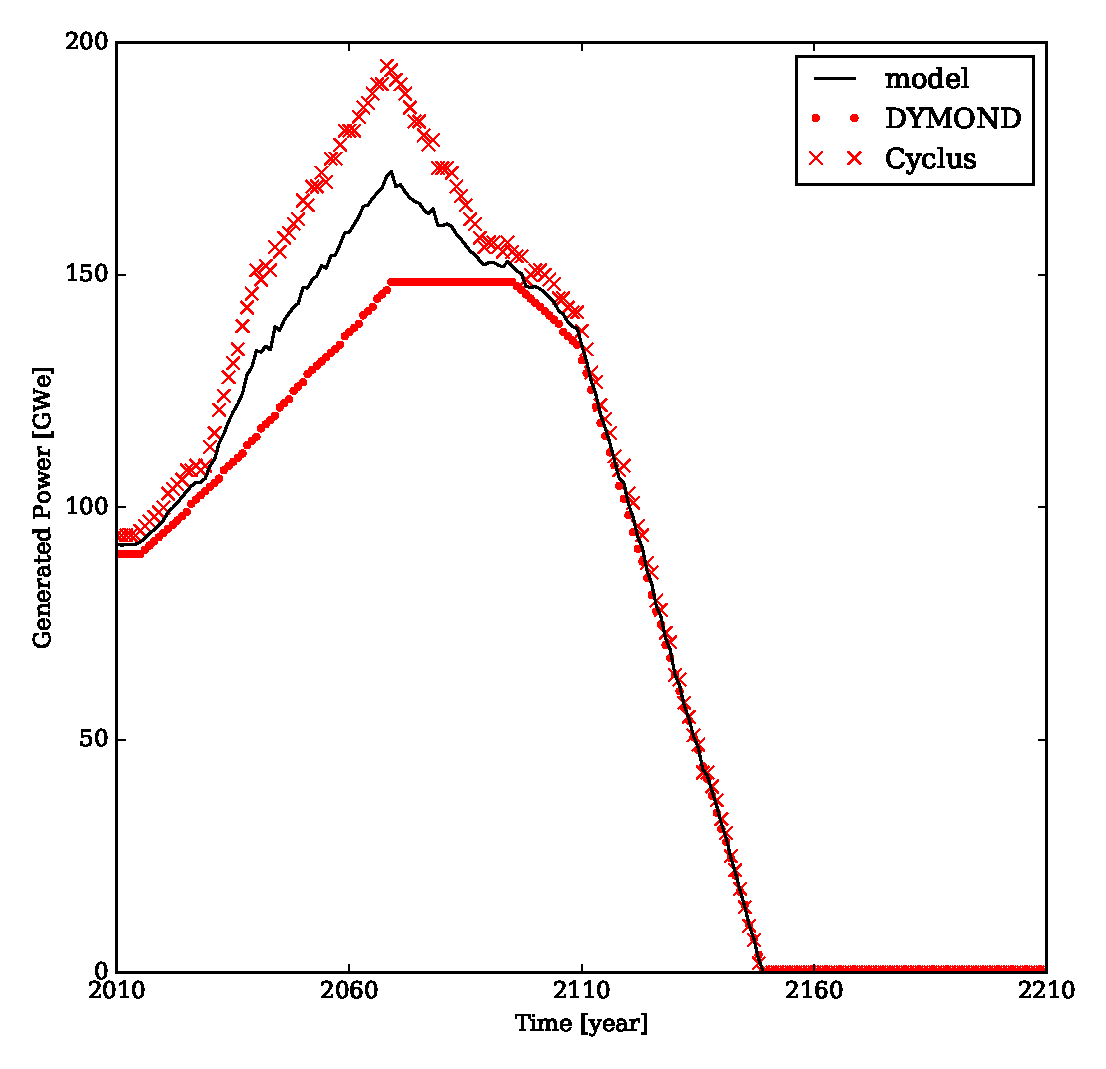
\includegraphics[width=0.9\textwidth]{gwe-model-lwr.eps}
\caption{The Gaussian process model of the generated power from LWRs
as a function of time as well as the results from the simulator that served as a 
training set for the model.}
\label{gwe-model-lwr}
\end{figure}

\begin{figure}[htb]
\centering
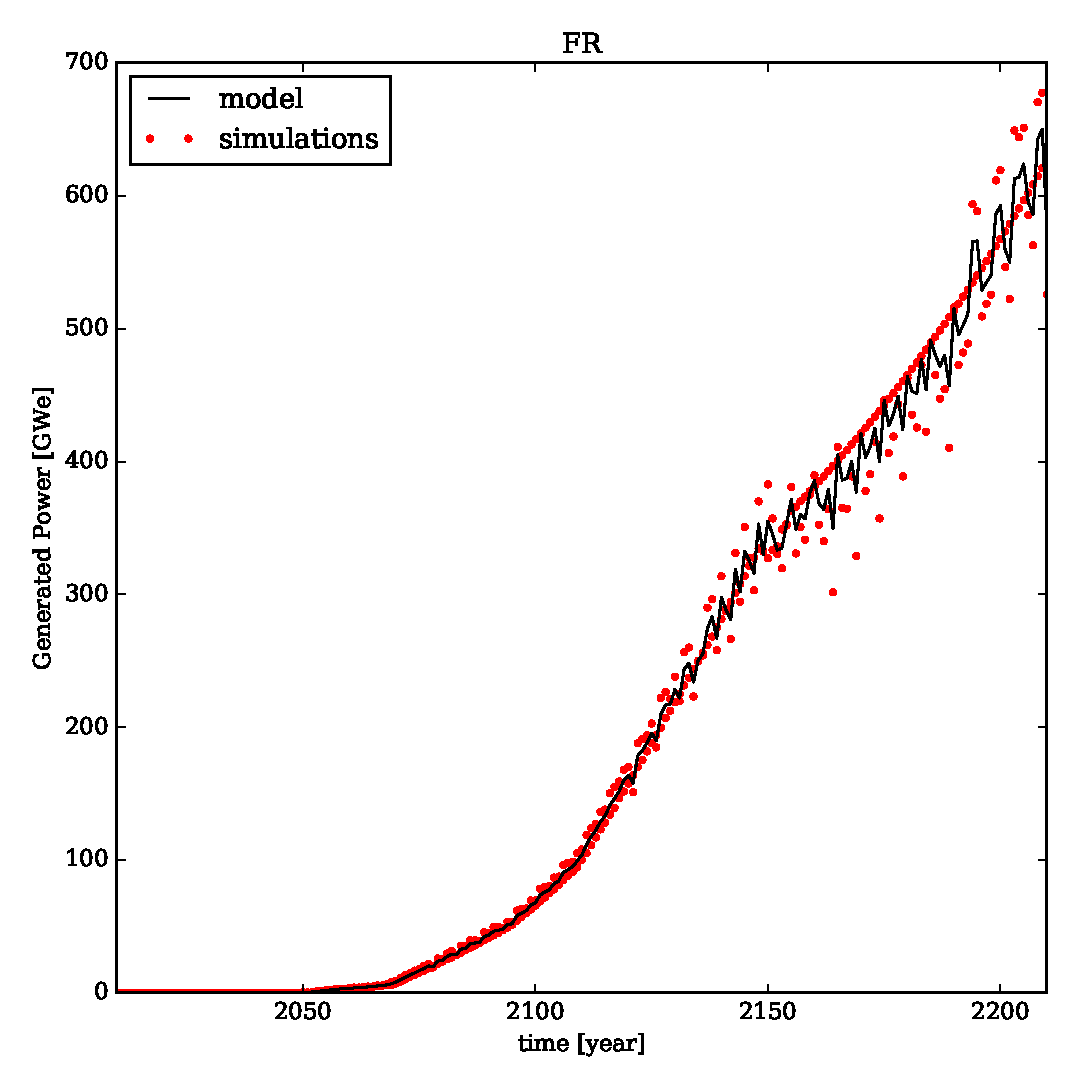
\includegraphics[width=0.9\textwidth]{gwe-model-fr.eps}
\caption{The Gaussian process model of the generated power from FRs
as a function of time as well as the results from the simulator that served as a 
training set for the model.}
\label{gwe-model-fr}
\end{figure}

\begin{figure}[htb]
\centering
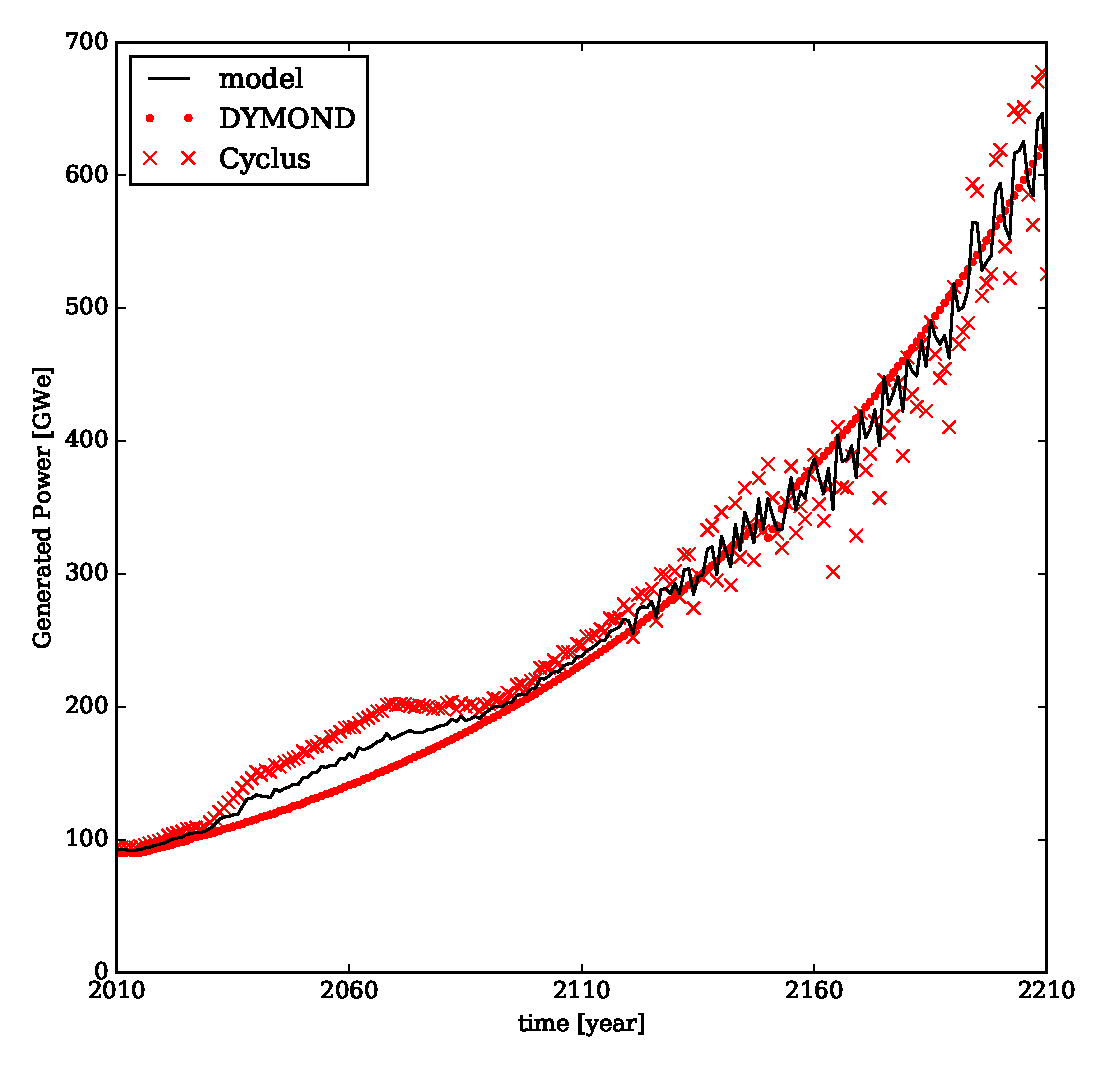
\includegraphics[width=0.9\textwidth]{gwe-model-total.eps}
\caption{The Gaussian process model of the total generated power
as a function of time as well as the results from the simulator that served as a 
training set for the model.}
\label{gwe-model-total}
\end{figure}

\clearpage

Also note that Figure \ref{gwe-model-total} displays the model of the total 
generated power and not the total of the constituent models. Symbolically, 
\begin{equation}
\label{total-model}
m_* \approx \GP \left[\sum_i^I m_s^i\right] \ne \sum_i^I \GP m_s^i
\end{equation}
This is because the uncertainties are applied differently in these two cases. 
Moreover, the hyperparameter
optimization would not be consistent if one were to sum up constituent 
models. It is thus considered safer
to sum over the features for each simulator individually before applying the 
regression.

Thus far the metric data has had effectively zero uncertainty, but one of the 
desirable features of the Gaussian process regression is that it may account
for uncertainties. As a thought experiment, suppose that the time 
series data happened to be much sparser and that 
the uncertainty associated with each value started off at zero and then grew at 
a rate of 1\% per decade. A model of the total generated power with this uncertainty 
is shown in Figure \ref{gwe-model-total-with-uncertainty}.

\begin{figure}[htb]
\centering
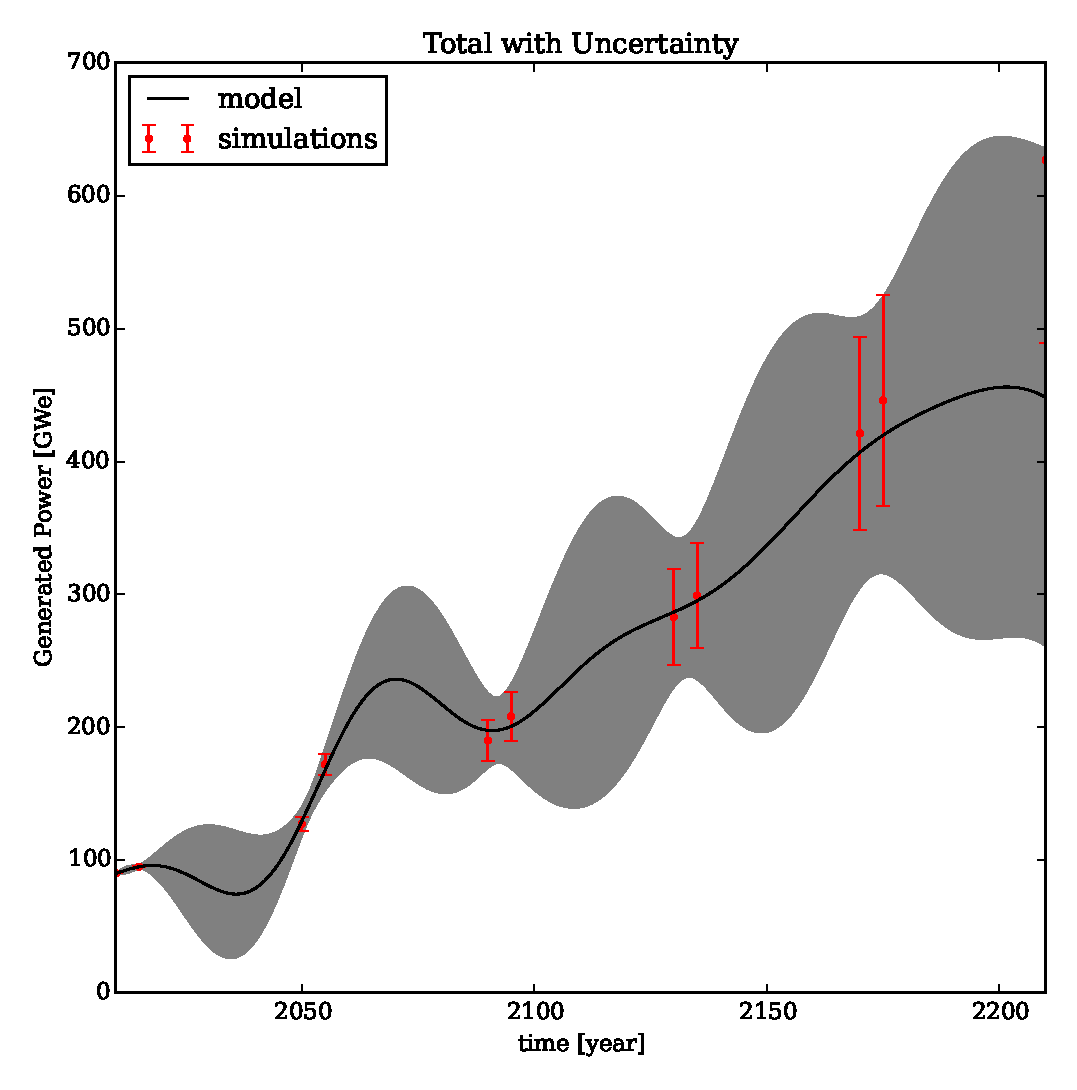
\includegraphics[width=0.9\textwidth]{gwe-model-total-with-uncertainty.eps}
\caption{The Gaussian process model of the total generated power
as a function of time. The training set data is relatively sparse and its uncertainty
has a 1\% per decade growth rate. The model curve is evaluated at every year. The 
gray envelope represents two standard deviations from the model, as computed by 
the Gaussian process.}
\label{gwe-model-total-with-uncertainty}
\end{figure}

In Figure \ref{gwe-model-total-with-uncertainty}, note that as the model moves 
farther in time from the training data the standard deviation grows. Furthermore, 
as the uncertainty in the training data grows, the model itself degrades. Artifacts
from the choice of kernel begin to be visible in model whenever the uncertainties are 
relatively high. Both of these match intuition about how uncertain systems should
work.

Again, even though these uncertainty features are highly desirable in 
generic benchmarking applications, most nuclear fuel
cycle simulators do not report uncertainties along with the metrics they compute.
For this reason, the remainder of the examples in the paper will use the 
zero-uncertainty models as presented in Figures \ref{gwe-model-lwr} - 
\ref{gwe-model-total}.


